\section{Calibration} \label{sec:calib}

In this section the various calibration procedures taken in order to minimize the time resolution and enhance both the particle identification (PID) and time of flight (TOF) capabilities of the Start Counter are discussed.

\subsection{Time-Walk Correction} \label{sec:calib_tw}

The time-walk effect is a well understood consequence of leading edge discriminators (LED).  Analog signals of varying amplitudes crossing a fixed threshold, as determined by the discriminator threshold setting, will do so at varying times as can be seen Fig.~\ref{fig:time_walk_effect}.
\begin{figure}[!htb]
	\centering
	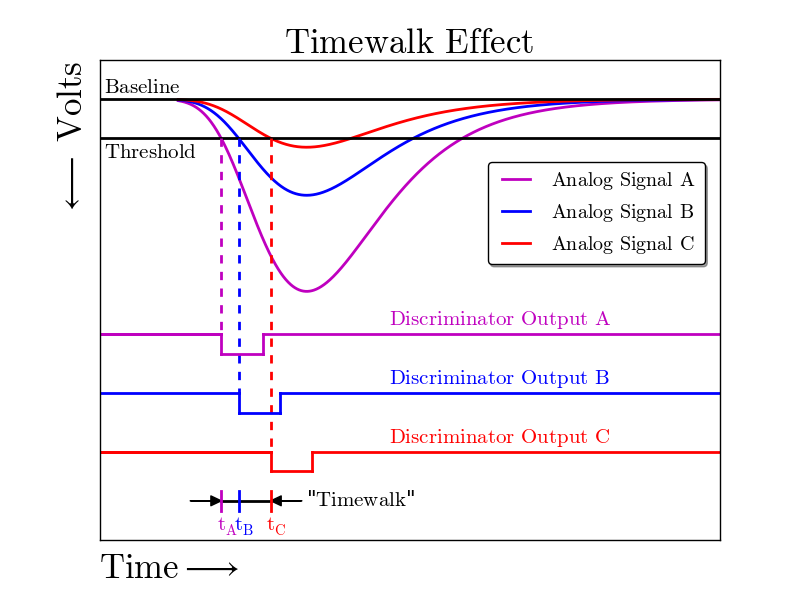
\includegraphics[width=1.0\columnwidth]{calibration/figs/time_walk_effect}
	\caption{Example of the time-walk effect. Three coincident analog signals A, B, \& C of varying amplitudes crossing a fixed threshold in a LED. The discriminator logic output signals vary in time relative to the amplitude of the incoming analog signal.  The signals shown above are simulated analog signals being fed into the LED's thus, they have negative polarity.}
	\label{fig:time_walk_effect}
\end{figure}
Thus, it is clear that the logic signal output from the discriminator ``\textit{walks about}'' in time, resulting in an undesirable smearing of time resolution of the ST TDC channels.

The FADC250's provide a high resolution pulse time (62.5~ps) that is time-walk independent \cite{pooser16} \cite{dong_fadc}.  
Therefore, for events in which both the FADC and TDC register hits in the same channel the pulse time can be used as a suitable reference time for that event. 